\documentclass[conference]{IEEEtran}
\usepackage{graphicx}
\usepackage{latexsym}
\usepackage{enumerate}
%\usepackage{ascmac}
\usepackage{url}
%\usepackage{fancybox}
%\usepackage{subfigure}
\usepackage{mediabb}

\graphicspath{{./figures/}}
\newcommand{\figref}[1]{Figure \ref{#1}}
\newcommand{\tabref}[1]{Table \ref{#1}}
\newcommand{\secref}[1]{Section \ref{#1}}

\hyphenation{op-tical net-works semi-conduc-tor}

\begin{document}

\title{ROCAT on KATARIBE:\\ Code Visualization for Communities}

\author{
\IEEEauthorblockN{
Tomohiro Ichinose\IEEEauthorrefmark{1},
Kyohei Uemura\IEEEauthorrefmark{1},
Daiki Tanaka\IEEEauthorrefmark{1},
Hideaki Hata\IEEEauthorrefmark{1},
Hajimu Iida\IEEEauthorrefmark{1},
Kenichi Matsumoto\IEEEauthorrefmark{1}
}

%\IEEEauthorblockN{
%Yusuke Saito\IEEEauthorrefmark{1},
%Shin Fujiwara\IEEEauthorrefmark{1},
%Kenji Fujiwara\IEEEauthorrefmark{1},
%Stevche Radevski\IEEEauthorrefmark{1},\\
%Hideaki Hata\IEEEauthorrefmark{1},
%Hajimu Iida\IEEEauthorrefmark{1},
%Kenichi Matsumoto\IEEEauthorrefmark{1}
%}
\IEEEauthorblockA{\IEEEauthorrefmark{1}Graduate School of Information Science,
Nara Institute of Science and Technology\\
Takayama-cho 8916-5, Ikoma-shi, Nara,
630-0192 Japan\\
Email: \{ichinose.tomohiro.ik1@is, uemura.kyohei.ub9@is, tanaka.daiki.sx4@is, hata@is, iida@itc, matumoto@is\}.naist.jp}
}
%Email: \{saito.yusuke.sl9, fujiwara.shin.fe5, kenji-f, stevche.radevski.sl1, hata\}@is.naist.jp,\\
%iida@itc.naist.jp, matumoto@is.naist.jp}
%}

\maketitle

\begin{abstract}
As globally distributed software development have been generalized, social coding platform like Github is needed for collaboration in a team. To share and help understand the overview of projects among teams, source code visualization is said to be useful.
In this paper, we present a new visual software development tool, Rocat, a code city like software visualization in virtual reality. In addition, we integrate Rocat with GitLab-based code hosting service, Kataribe. By integrating Rocat into Kataribe, fine-grained code information can be visualized, and sharing the city visualization can be easily available. We present our tool and the provided features of Rocat on Kataribe.
A Screencast for demonstration is available at the following URL.\\
\url{https://www.youtube.com/watch?v=ZQTTO91v4No}
\end{abstract}



\section{Introduction}
Since the beginning of software development, the size and complexity of software have been continuously on the rise.
If the software for a space shuttle 30 years ago was 400,000 lines of code, nowadays even a smartphone application can easily exceed that size.
Not only the size of software increased in terms of LOC, but the integration and interaction with external services dramatically increased.
With the increase of size and complexity, it gets more and more difficult to comprehend the structure and analytics of software, especially without a good way to visualize the information.

One good way to represent the software structure, size, and modularity is CodeCity \cite{Wettel:2011:SSC:1985793.1985868}, representing classes as buildings, and packages as districts in 3D, synonymous to a city.
Since the original CodeCity does not offer a great number of interactions a developer can do with the city, there has been some work to extend it.
One interesting approach is CodeMetropolis \cite{6648194}, where they represent software cities in Minecraft, allowing for better collaboration within the Minecraft game.
Showing similar data as CodeCity, CodeMetropolis allows the user to walk around the city and interact closely with the buildings (that is the source code).
The same representation has also been used to specifically represent the development history using a bird-eye view of the city \cite{Steinbruckner:2010:RDH:1879211.1879239}.
Each one having its own purpose, they assist in the understanding of software.

\begin{figure}[h]
\centering
\includegraphics[width=8cm]{NewRocat.pdf}
\caption{City-like code visualization}
\label{figure:new-Rocat}
\end{figure}

The reason we believe these visualization techniques are very good is because of the ease to understand the structure of the software, the classes size, and the number of packages within seconds.
Furthermore, humans are very good at processing very large amount of information in the real-world city like views very fast, since we learn and adapt to the environment we live in.
For example, just by glancing over a building, you can tell how old the building is, whether it is a modern or classic design, the material it is made of, the color, and much more.
That being said, using a visualization technique that is synonymous with the real-world allows us to map the meanings of characteristics from the real-world to some aspect of the software, processing it with a similar speed as we would process the meaning of the real-world object.

Even though we believe the previously mentioned approaches are great to visualize software, we think that the full potential of such visualization technique is not utilized.
They use the concepts of a city to some extent, but they have not included many other aspects that real cities have and that can be used to deliver even more information to software engineers.
If we manage to grasp this potential and use it in a way that is consistent with how we process information in the real environment, understanding the elements of a software system will get much faster and deeper.

Because of that, our aim is to bring software cities reflect real cities in many other ways.
We want to provide an experience where the software engineer is immersed in the software, exploring it and learning (maybe even subconsciously) about it while walking around, in the same way as one would explore a real city.
We want to allow the engineer to naturally interact with the information and source code the software has, hoping that such enriched experiences should help in better retention of information, as well as easier comprehension.
To realize such system, we present a visualization tool, \textit{Rocat}, which shows city-like code visualization in virtual reality environment.

\begin{figure*}[t!]
\centering
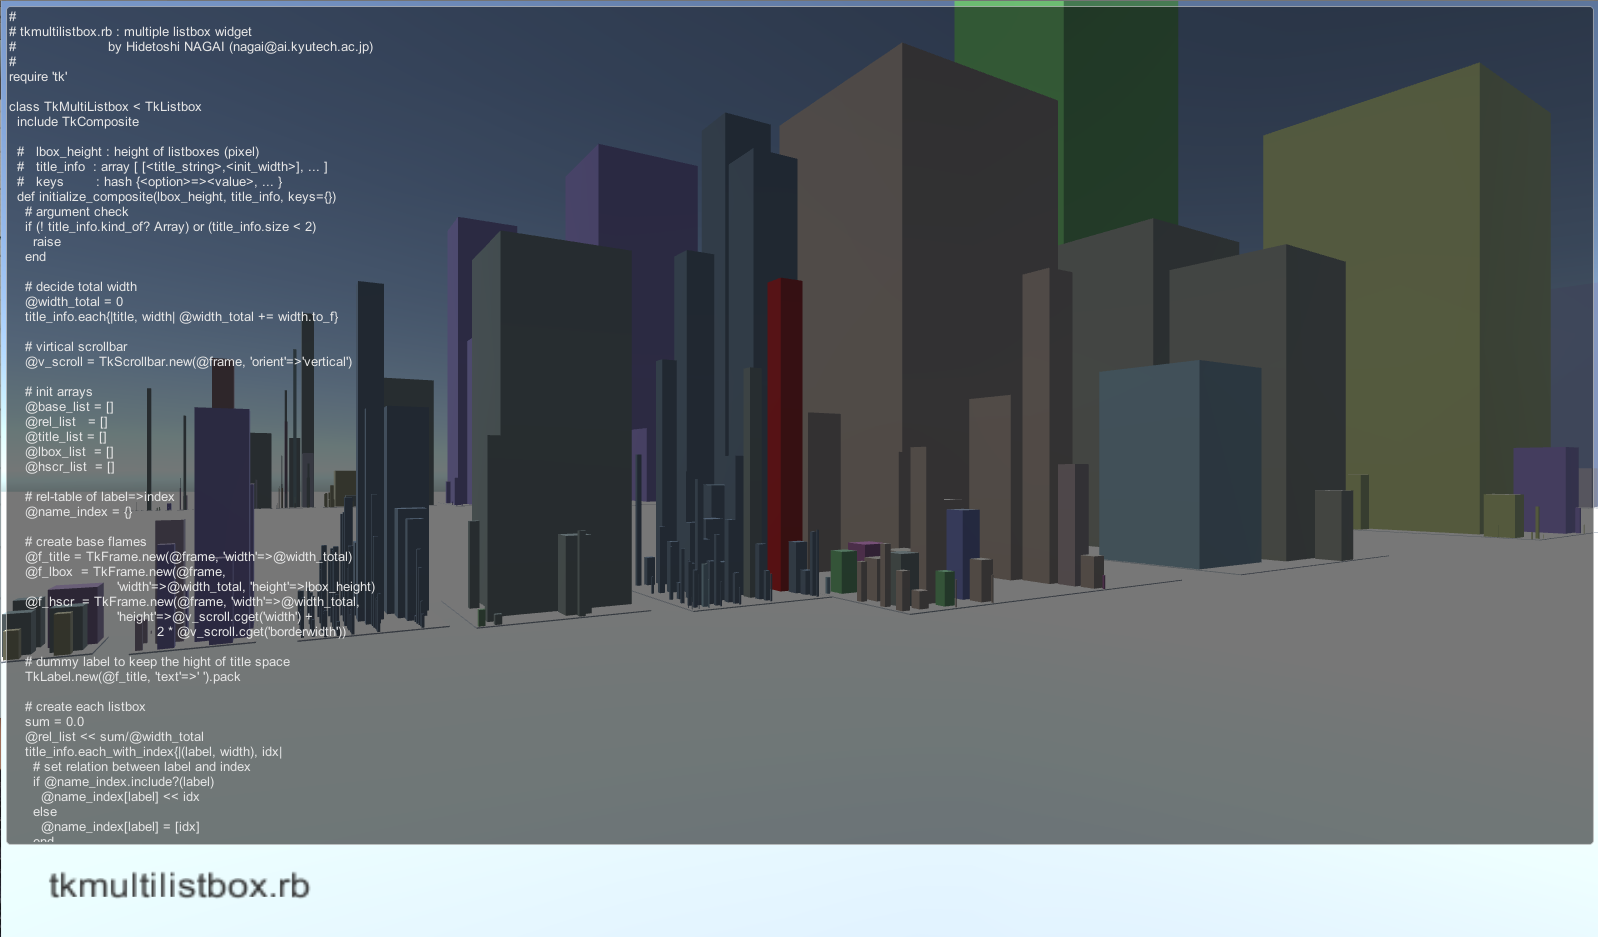
\includegraphics[bb=0 0 1598 937, width=18cm]{rocat.png}
\caption{Snapshot of Rocat}
\label{figure:Rocat}
\end{figure*}

\begin{figure}[tb]
\centering
\includegraphics[width=8cm]{Rocat-on-kataribe2.pdf}
\caption{Snapshot of Rocat on Kataribe}
\label{figure:Rocat-on-kataribe}
\end{figure}


In addition, we want to introduce the new concept of code visualization, that is, code visualization for communities.
Previous visualization tools mainly focused on supporting developers, a single developer \cite{Wettel:2011:SSC:1985793.1985868} or a team of developers \cite{6648194}.
However, we think that visualization should be beneficial for communities too, as we've learned the effectiveness of social coding \cite{Dabbish:2012:SCG:2145204.2145396} and pull-based development \cite{Gousios:2014:ESP:2568225.2568260}.
To address this challenge, we integrated Rocat on \textit{Kataribe},  our code hosting service.
With this kind of system, communities can share a large amount of information about the underlying software in a way that is quick and easy to understand.

\section{Rocat: Software Visualization}
To support developers comprehend source code and the conditions of projects, we propose \textit{Rocat}, where developers can feel the code as a city, and provide richer experiences by enabling exploring the city.
If the information represented on the building (or city) and their meaning is synonymous with the real-world city, it will be easy to quickly retrieve the meaning they carry.
In this section, we describe the overview and implementation of Rocat and inform the concept of further usage.

\subsection{Overview and Implementation}
Rocat is a visualization tool that can be applied to multiple software development environments.
\figref{figure:Rocat} presents the snapshot of Rocat view.
Similar to the CodeCity \cite{Wettel:2011:SSC:1985793.1985868}, extracted metrics are mapped on the hight and the base size of buildings.
Users can explore the city among buildings.
When one building is selected (red building in the figure), its source code can be available on demand.
It is possible to edit this source code with this view.
The color of the building describes the top contributor of the file corresponds to the building.
These color can be used to find out who understand and has a responsible for certain source code file.

Although CodeMetropolis is realized on top of an attractive popular role-playing game, Minecraft\footnote{\url{https://minecraft.net/}} \cite{6648194}, we have started implementation using a cross-platform game engine, Unity\footnote{\url{https://unity3d.com/}}.
This is because we want not to limit Rocat to specific purposes, and want to develop general software development platform in the future.
By using Unity, Rocat can be run on a web browser or any platform and can adopt Oculus Rift to see Rocat in virtual reality.

Rocat is not the only visualization but intends to a novel software development environment.
We describe our concept with the following related approach.


\subsection{Concept}
\subsubsection{Virtual Museum}
A virtual museum is a digital entity that draws on the characteristics of a museum, in order to complement, enhance, or augment the museum
experience through personalization, interactivity and richness of content\footnote{\url{https://en.wikipedia.org/wiki/Virtual_museum}}.
Storytelling is one of the aims of virtual museums, which intends to make cultural content more attractive for the public and, consequently, the leaning process easier \cite{Pietroni:2014:IVR:2635823.2611375}.
This aim is also important for Rocat.

\subsubsection{Web Maps}
Web maps like Google Maps\footnote{\url{https://maps.google.com/}} are indispensable for exploring real world cities.
Among various useful features, a zooming feature is one of basic and essential one to comprehend the structure of cities.
Rocat provides hierarchical views from a bird-eye view to an exploring view.
From bird-eye views, we can glance the characteristics of entire or part of projects.
With exploring views, we can investigate each building with considering neighbors.

\subsubsection{Visual Software Analytics Platform}
Software analytics is analytics on software data for managers and software engineers with the aim of empowering software development individuals and teams to gain and share insight from their data to make better decisions \cite{Menzies:2013:SAS:2553351.2553360} SAMOA is a visual software analytics platform \cite{6676936}.
As a software development environment, Rocat also needs to help decision making, that is, Rocat can be a visual software analytics system too.
SAMOA is 2D system and has different views: a snapshot view, an evolution view, and an ecosystem view.
Introducing these kinds of views in 3D environments might be helpful.

\subsubsection{Team Collaboration Platform}
From an empirical study of modern code review, Bacchelli and Bird reports the motivations of code review \cite{Bacchelli:2013:EOC:2486788.2486882}. While finding defects remain the main motivation, reviewers also expect additional benefits such as knowledge transfer, increased team awareness, sharing code ownership, and so on.
To support these outcomes, Rocat can be helpful, that is, Rocat can be team collaboration platform too.

\section{Kataribe: Fine-grained Code Hosting}
\textit{Kataribe}\footnote{http://kataribe-dev.naist.jp} is a hosting service of Historage repositories \cite{Fujiwara:2014:KHS:2597073.2597125}.
Historage repositories are fine-grained source code repositories \cite{Hata:2011:HFV:2024445.2024463}, and are converted from file-level Git repositories with a tool, \textit{Kenja}\footnote{\url{http://github.com/niyaton/kenja}}.
Kenja constructs a directory structure for the Historage based on the result of syntactic analysis of all source code files in each commit.
Currently, Kataribe hosts Historage written in C\#, Go, Python and Ruby, since Kenja can only construct on those programming languages.
Kataribe uses Gitlab, which is a well-known OSS for hosting Git repositories.
Users can get Historage repositories from Kataribe without registration.
Registration at Kataribe enables users to browse Historage repositories on the web.
Gitlab enables users to see logs and graphical statics of repositories.

Features of Kataribe include importing existing Git repositories that are provided on Git hosting services such as Github and also constructing Historage repositories incrementally.
Since a Historage repository created by Kenja is separated from the original repositories, users of Kataribe can continue their development regardless of their Historage repositories.
When developer pushes her/his commits into their original repositories, Kataribe automatically converts pushed commits into the corresponding Historage repositories.
These features allow researchers to get latest fine-grained histories when they want to start their new research.

\section{Rocat on Kataribe}
We have integrated Rocat into Kataribe to provide software analytics for the community.
\figref{figure:Rocat-on-kataribe} shows a screen capture of Rocat on Kataribe.
Kataribe provides Rocat page, which can be seen by pressing the tab button seen in the upper menu, for each repository.
The bottom half shows the current source code which corresponds with building selected by the user.

Rocat on Kataribe runs by Unity Web Player\footnote{http://unity3d.com/webplayer}, one of the supported platform by Unity for executing the project on a web browser.
The metrics data for constructing the building are managed on Kataribe, so updating the city and each building can be easily performed.
In addition, data and source code shown by Rocat are always updated to the newest version.

Since Kataribe uses Gitlab, not only developers but also user without registration are able to look through the overview of the project by Rocat.
This characteristic of sharing visualization in public differs from the prior studies and tools which targeted single developer or project team.
Also, integrating Rocat to source code hosting service, the user no need to care about doing extra work to share the visualization and can concentrate on their work.
To make better use of Kataribe, using the Historage metrics to construct the building can be done.
Metrics includes in Historage helps user for more in-depth analysis and extend the possibilities for more understandable visualization.

% For the further evolution of Rocat on Kataribe, supporting real-time discussion and expressing software evolution could be conceivable.

\begin{figure}[tb]
\centering
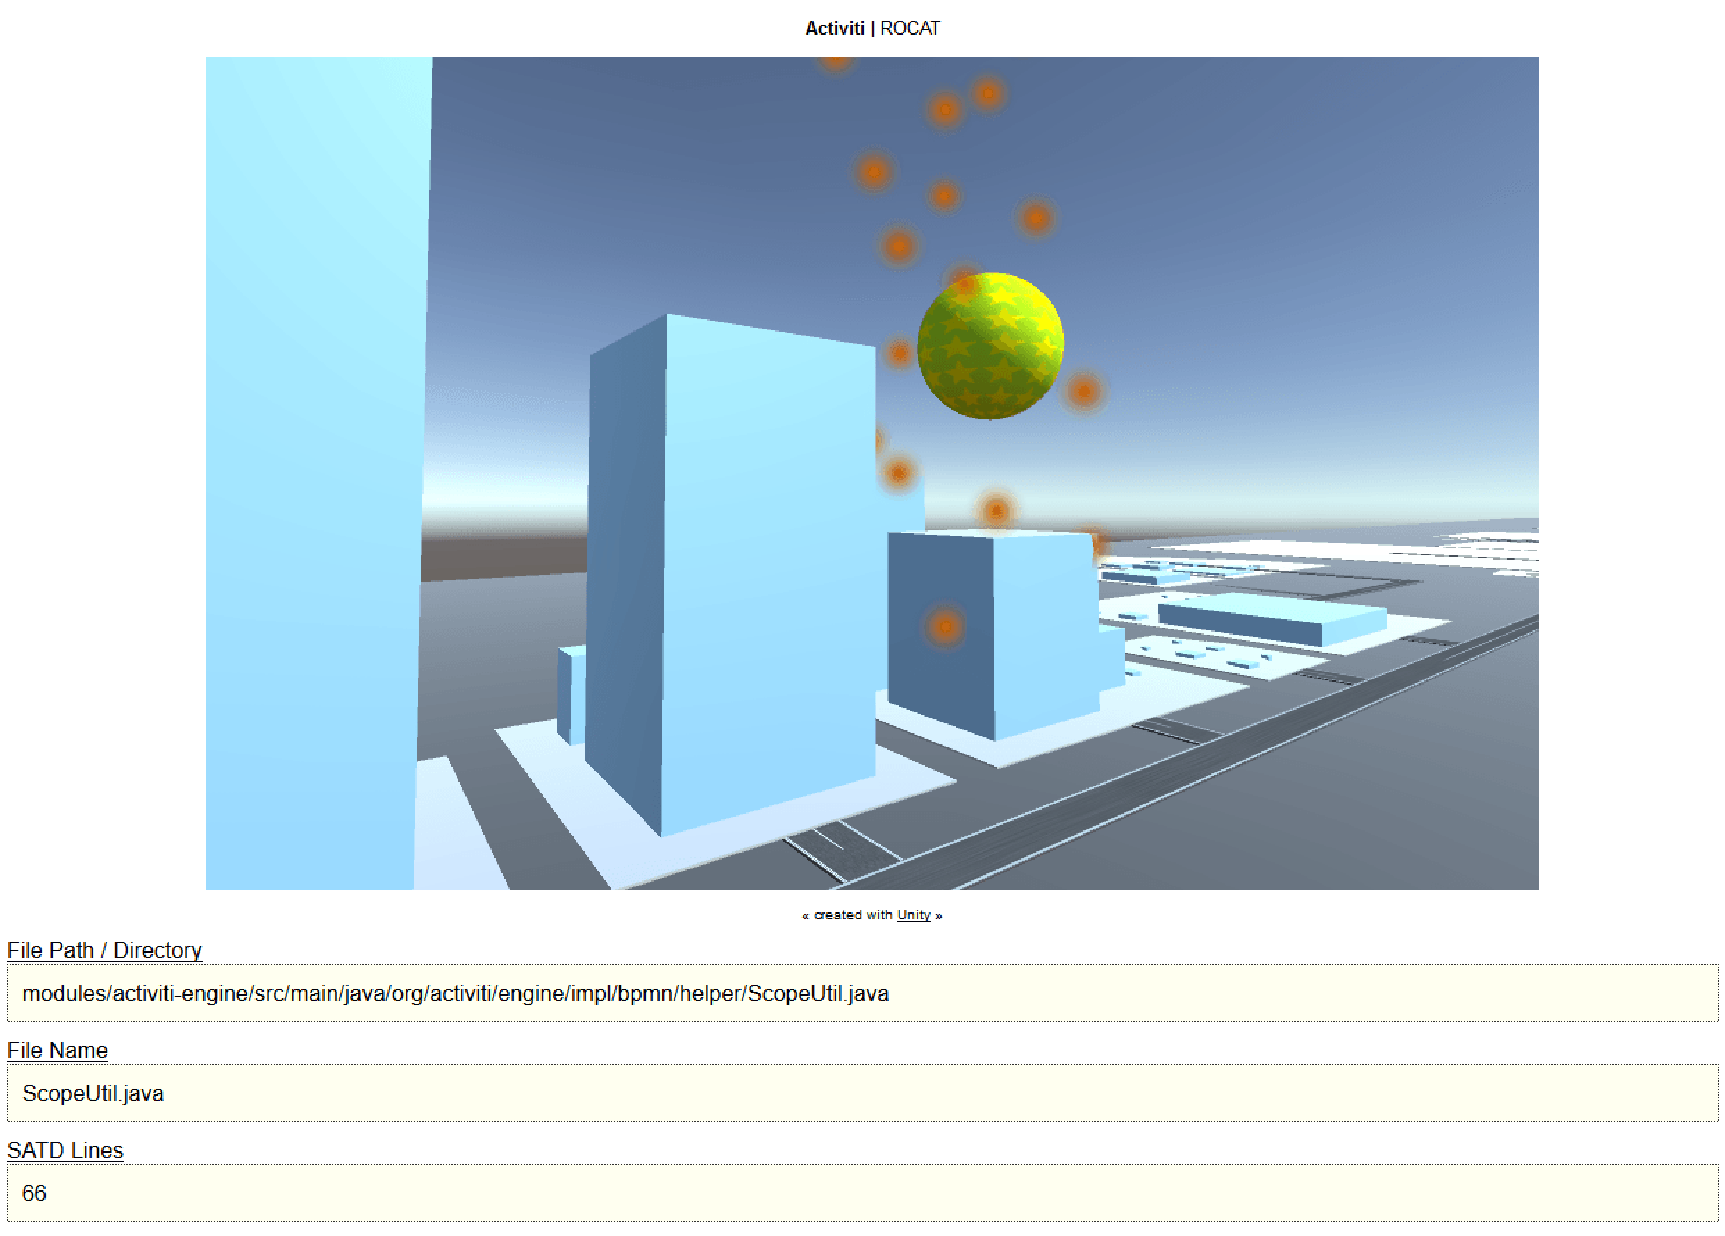
\includegraphics[width=8cm]{satd.pdf}
\caption{Visualization for self-admitted technical debt}
\label{figure:SATD}
\end{figure}

\section{Discussions and Future Work}
We strongly believe that visualization is a crucial part of successful software engineering.
Although currently some topics are separately studied like software analytics, team collaboration, learning/comprehension, knowledge sharing, and so on, we think that visual environment can be the center of these issues.
We are developing a system using Rocat that visualizes self-admitted technical debt (SATD).
Technical debt is a metaphor that has been used to express non-optimal solutions of software development, and SATD is a kind of technical debt that is intentionally introduced into source code with keywords such as "TODO" or "FIXME".
\figref{figure:SATD} shows a screen capture of the system.
The green ball and orange bubbles are markers of SATD.
The users can find files that contain SATD without reading source codes and share the information that which file should be done refactoring.

This paper presents code city for multiple software development environments, named Rocat.
From here on, we continue to develop Rocat for building a new visual software development environment.
To start with, we also present Rocat on Kataribe for providing software analytics for communities.

\section*{Acknowledgment}
This work has been supported by JSPS KAKENHI Grant Number 26540029, and Program for Advancing Strategic International Networks to Accelerate the Circulation of Talented Researchers: Interdisciplinary Global Networks for Accelerating Theory and Practice in Software Ecosystem.
We would like to thank Takao Nakagawa for the suggestions about the demo movie.



\bibliographystyle{IEEEtran}
\bibliography{ref,reference-hata}

\end{document}
